%%%%%%%%%%%%%%%%%%%%%
%% MEDICAL IMAGING %%
%%%%%%%%%%%%%%%%%%%%%
\section{Experiments on Medical Imaging Datasets}
\label{sec:real}

% \begin{table}[!t]
\caption{
Mean Squared Error on unseen test data, $5$-fold cross validation.
Mean (standard deviation) across folds are shown. Best results in boldface.
Test data may belong to the same datset used to train the model (within) or on all the other (cross).
Every modality was predicted from the other available ones.
}
\centering
\begin{tabular}{llcccccc}
\toprule
             &       &         clin &          mri &          fdg &         av45 &          tau &   mri local \\
train & test &              &              &              &              &              &              \\
\midrule
adni1 & within &  0.91 (0.11) &  0.95 (0.13) &            - &            - &            - &            - \\
             & cross &  0.91 (0.29) &  1.01 (0.44) &            - &            - &            - &            - \\
\midrule
adni2 & within &  0.77 (0.11) &  \textbf{0.91} (0.20) &  \textbf{0.82} (0.20) &  \textbf{0.93} (0.22) &  1.20 (0.71) &            - \\
             & cross &  0.82 (0.27) &  1.00 (0.41) &            - &  1.28 (0.46) &  1.67 (1.19) &            - \\
\midrule
miriad & within &  0.74 (0.34) &  1.01 (0.52) &            - &            - &            - &            - \\
             & cross &  0.89 (0.15) &  0.99 (0.18) &            - &            - &            - &            - \\
\midrule
local & within &  0.94 (0.28) &            - &            - &  1.20 (0.28) &  1.43 (1.29) &  \textbf{1.23} (0.35) \\
             & cross &  1.29 (0.28) &            - &            - &  1.13 (0.24) &  \textbf{1.17} (0.75) &            - \\
\midrule
\midrule
average & within &  0.84 (0.21) &  0.96 (0.29) &  \textbf{0.82} (0.20) &  1.06 (0.25) &  1.32 (1.00) &  \textbf{1.23} (0.35) \\
        & cross  &  0.98 (0.25) &  1.00 (0.34) &            - &  1.21 (0.35) &  1.42 (0.97) &            - \\
\midrule
\midrule
% all (dae)        & within &  0.56 (0.05) &  1.02 (0.12) &  0.98 (0.24) &  1.02 (0.17) &  1.11 (0.62) &  1.10 (0.34) \\
% all (knn5)        & within &  \textbf{0.65} (0.04) &  1.03 (0.11) &  1.09 (0.20) &  1.42 (0.17) &  1.29 (0.66) &  \textbf{1.23} (0.38) \\
all       & joint &  \textbf{0.65} (0.05) &  0.95 (0.12) &  0.85 (0.21) &  0.99 (0.20) &  \textbf{1.17} (0.64) &  1.25 (0.35) \\
\bottomrule
\end{tabular}
\label{table:crossvalidation_details}
\end{table}

%\begin{table}[!t]
%\caption{
%Same as above, after average-pooling af means and standard deviations by 
%}
%\centering
%\begin{tabular}{lcccccc}
%\toprule
%{} &         clin &          mri &          fdg &         av45 &          tau &   mri local \\
%train/test   &              &              &              &              &              &              \\
%\midrule
%within &  0.84 (0.21) &  0.96 (0.29) &  0.82 (0.20) &  1.06 (0.25) &  1.32 (1.00) &  1.23 (0.35) \\
%cross  &  0.98 (0.25) &  1.00 (0.34) &            - &  1.21 (0.35) &  1.42 (0.97) &            - \\
%joint  &  0.65 (0.05) &  0.95 (0.12) &  0.85 (0.21) &  0.99 (0.20) &  1.17 (0.64) &  1.25 (0.35) \\
%\bottomrule
%\end{tabular}
%\label{table:crossvalidation}
%\end{table}


% \begin{sidewaystable}
\centering
\begin{tabular}{llllllll}
\toprule
       &      &         clin &           mri &          fdg &         av45 &          tau &   mri\_geneva \\
test dataset & train type &              &               &              &              &              &              \\
\midrule
adni1 & within &  0.90 (0.12) &   0.95 (0.16) &            - &            - &            - &            - \\
       & cross &  1.17 (0.80) &   2.88 (3.10) &            - &            - &            - &            - \\
       & lodo &  0.46 (0.07) &   1.13 (0.16) &            - &            - &            - &            - \\
\midrule
adni2 & within &  0.78 (0.12) &   0.91 (0.24) &  0.85 (0.25) &  0.94 (0.27) &  1.24 (0.93) &            - \\
       & cross &  1.08 (0.64) &   2.17 (2.12) &  4.03 (0.85) &  3.34 (2.65) &  1.33 (0.97) &            - \\
       & lodo &  0.60 (0.29) &   0.81 (0.21) &  3.90 (0.90) &  3.04 (2.52) &  1.10 (0.74) &            - \\
\midrule
miriad & within &  0.76 (0.47) &   1.01 (0.66) &            - &            - &            - &            - \\
       & cross &  7.20 (5.07) &  10.39 (4.47) &            - &            - &            - &            - \\
       & lodo &  2.32 (0.95) &   7.97 (2.14) &            - &            - &            - &            - \\
\midrule
geneva & within &  0.89 (0.33) &             - &  1.15 (0.47) &  1.25 (0.37) &  1.86 (3.04) &  1.20 (0.47) \\
       & cross &  2.69 (1.28) &             - &  6.09 (1.95) &  2.57 (3.04) &  2.36 (2.34) &            - \\
       & lodo &  1.83 (0.90) &             - &  5.99 (1.81) &  1.63 (0.48) &  2.47 (2.51) &            - \\
\midrule
oasis3 & within &  0.71 (0.15) &   0.81 (0.11) &            - &  1.10 (0.42) &            - &            - \\
       & cross &  1.29 (0.74) &   2.43 (2.47) &            - &  1.56 (0.93) &            - &            - \\
       & lodo &  0.76 (0.08) &   0.77 (0.11) &            - &  1.74 (0.34) &            - &            - \\
\bottomrule
       & within &  0.81 (0.24) &  0.92 (0.29) &  1.00 (0.36) &  1.10 (0.35) &  1.55 (1.98) &  1.20 (0.47) \\
       & cross  &  2.69 (1.71) &  4.47 (3.04) &  5.06 (1.40) &  2.49 (2.21) &  1.85 (1.66) &            - \\
       & lodo   &  1.19 (0.46) &  2.67 (0.66) &  4.94 (1.35) &  2.14 (1.11) &  1.79 (1.63) &            - \\
\bottomrule
\end{tabular}
\end{sidewaystable}

% \begin{table}[!t]
\caption{
Mean Squared Error (MSE) of test data from adni2.
All models were trained on all the available datasets by holding-out data from the adni2 test dataset.
$5$-folds cross validation of MSE is shown as mean (standard deviation).
Best results in boldface are significant with an $\alpha$ level of 0.01 with respect to both competing methods.
}
\centering
\label{tab:model_comparison}
\begin{tabular}{lccc}
\toprule
View       &          \multicolumn{3}{c}{model}\\
           &          dae &         knn5 &           ours        \\ \cline{2-4}
clin       &  0.73 (0.14) &  0.44 (0.05) &          0.45 (0.07) \\
MRI        &  1.23 (0.31) &  0.88 (0.15) &  \textbf{0.70} (0.13) \\
FDG        &  4.20 (0.56) &  4.15 (0.59) &  \textbf{1.09} (0.15) \\
AV45       &  1.45 (0.35) &  1.20 (0.25) &  \textbf{0.89} (0.15) \\
TAU        &  1.54 (0.82) &  1.44 (0.83) &  \textbf{1.05} (0.45) \\
\bottomrule
\end{tabular}
\end{table}

% \begin{table}[!t]
% \caption{
% Add OASIS3 dataset (clin, mri, av45)
% }
% \centering
% \begin{tabular}{lcccccc}
% \toprule
% model &         clin &          mri & fdg &         av45 &          tau & mri local \\
% % model &              &              &     &              &              &            \\
% \midrule
% knn5              &  0.50 (0.06) &  0.92 (0.13) &   - &  \textbf{1.33} (0.23) &  1.10 (0.54) &  -  \\
% dae               &  0.45 (0.08) &  0.95 (0.15) &   - &  1.49 (0.20) &  1.09 (0.50) &  -  \\
% our               &  \textbf{0.39} (0.05) &  \textbf{0.75} (0.13) &   - &  1.38 (0.21) &  \textbf{0.93} (0.51) &  -  \\
% \bottomrule
% \end{tabular}
% \label{table:model_comparison}
% \end{table}
% 
% \begin{table}[!t]
% \caption{
% Add OASIS3 dataset (clin, mri, av45), ComBat normalize (mri, fdg, av45, tau)
% }
% \centering
% \begin{tabular}{lcccccc}
% \toprule
% model &         clin &          mri & fdg &         av45 &          tau & mri local \\
% % model &              &              &     &              &              &            \\
% \midrule
% knn5              &  0.51 (0.07) &  1.10 (0.17) &   - &  1.16 (0.19) &  \textbf{1.08} (0.62) &  -  \\
% dae               &  0.44 (0.06) &  1.09 (0.17) &   - &  \textbf{1.06} (0.19) &  1.45 (0.70) &  -  \\
% our               &  \textbf{0.42} (0.05) &  \textbf{0.94} (0.15) &   - &  \textbf{1.06} (0.20) &  1.32 (0.71) &  -  \\
% \bottomrule
% \end{tabular}
% \label{table:model_comparison}
% \end{table}
% 
% \begin{table}[!t]
% \caption{
% Add OASIS3 dataset (clin, mri, av45), add Geneva PET, ComBat normalize (mri, fdg, av45, tau)
% }
% \centering
% \begin{tabular}{lcccccc}
% \toprule
% model &         clin &          mri & fdg &         av45 &          tau & mri local \\
% % model &              &              &     &              &              &            \\
% \midrule
% knn5              &  0.50 (0.06) &  1.09 (0.17) &   - &  1.18 (0.20)  &  1.23 (0.92)  &  -  \\
% dae               &  0.42 (0.08) &  1.09 (0.16) &   - &  1.08 (0.19)  &  1.54 (0.87)  &  -  \\
% our               &  \textbf{0.41} (0.06) &  \textbf{0.93} (0.15) &   - &  \textbf{1.07} (0.17)  &  \textbf{1.17} (0.81)  &  -  \\
% \bottomrule
% \end{tabular}
% \label{table:model_comparison}
% \end{table}


% Joint modeling of multiple datasets in real applications often represents an hybrid case between modeling missing at random (MAR) and missing not at random (MNAR) observations.
% Indeed, every dataset may lack of views which are instead present in others by default.
% At the same time, in each dataset, there may be missing views for some data-points due to unknown reasons.
% 
In this section we describe our results on jointly modeling real medical imaging datasets, independently acquired in the context of dementia studies.

We executed three kinds of experiments:
1) benchmark evaluation of our model against the best competing methods from the previous section;
2) multi-view feature prediction with our model on all the available datasets in multiple training and testing conditions.
3) diagnosis classification from multi-view heterogeneous data in different training and testing conditions.

\subsection{Data Sources}
\label{ssec:datasets}

Data used in the preparation of this section were obtained from the following sources.
\begin{enumerate}
%
\item The Alzheimer's Disease Neuroimaging Initiative (ADNI)
\footnote{
\href{http://adni.loni.usc.edu}{adni.loni.usc.edu}.
The ADNI was launched in 2003 as a public-private partnership, led by Principal Investigator Michael W. Weiner, MD. For up-to-date information, see \href{www.adni-info.org}{www.adni-info.org}.
},
a database of brain imaging and related clinical data of cognitively normal subjects, and on patients presenting various degrees of cognitive decline.
%
\item MIRIAD dataset, a database of brain imaging and related clinical data of cognitively normal subjects and patients affected by Alzheimer's disease \citep{Miriad}.
%
\item OASIS-3 dataset, a database of brain imaging and related clinical data of cognitively normal subjects and subjects at various stages of cognitive decline \citep{oasis3}.
%
\item A local cohort collected at the Geneva University Hospitals, with brain imaging and related clinical data of patients with various cognitive disorders.
\end{enumerate}
Subjects enrollment, data collection, and data sharing were approved by the ethic committees associated to each study dataset in accordance with the principles of the Declaration of Helsinki.
% Each subject, or his/her legal tutor, provided a voluntary written informed consent for participation in the original studies.

The available imaging modalities comes from the following acquisitions:
%
\begin{enumerate}
\item structural Magnetic Resonance Imaging (MRI) to measure anatomical volumes in the brain;
%
\item Positron Emission Tomography (PET) with Fluorodeoxyglucose (FDG) tracer, to measure the glucose uptake, which reflects the functional status of the brain;
\item PET with the AV45 tracer, to measure the amyloid deposits in the brain;
\item PET with the AV1451 tracer, to measure the tau protein aggregates in the brain.
\end{enumerate}
%

We divided the ADNI dataset into two complementary datasets:
`Adni1', composed by subjects recruited in the initial ADNI1 study (2004-2009),
and `Adni2' composed by those subjects subsequently recruited in ADNI-GO, ADNI2, and ADNI3 (2010-ongoing).
Data modalities and acquisition protocols of `Adni1' present differences from those of `Adni2'.
Specifically, in `Adni1' and `Adni2' the MRI imaging was performed respectively on 1.5T and 3T scanners.
The two cohorts differs also for the presence of PET imaging data.
Therefore we consider these two cohorts as separated datasets.

To summarize, we grouped our data into five distinct datasets which we named as follows: `Adni1', `Adni2', `Miriad', `Oasis3', `Geneva'.

\subsection{Imaging Processing}
The brain scans were processed in order to have measurements on regions defined in the Desikan-Killiany atlas \citep{Desikan2006}.
Brain MRI scans were processed with FreeSurfer \footnote{\href{https://surfer.nmr.mgh.harvard.edu/}{surfer.nmr.mgh.harvard.edu}} \citep{freesurfer} to measure brain cortical and sub-cortical volumes, and volumes occupied by the cerebro-spinal fluid (CSF), for a total of $99$ regions of interest.
Relative standardized uptake values (SUVR) were computed for the PET scans (FDG, AV45, AV1451), processed with SPM \citep{Ashburner2000}.
SUVRs were computed using the cerebellum as reference region, and averaged in the same regions used for the MRI, except those containing the CSF, for a total of $94$ regions of interest.

\subsection{Gathering Observations into Views}
\label{ssec:views}
\begin{table}[!t]
\caption{
Number of subjects per view available in each dataset.
The last columns provide the size of the intersection ($\cap$) and union ($\cup$) of subjects with available views.
The mri from the local dataset is considered as a stand-alone modality as the measures were obtained with a different protocol from the ones in the other datasets.
Notice how in the jont dataset no subject have all the modalities.
}
\centering
\resizebox{\columnwidth}{!}{
\begin{tabular}{lccccc|cc}
\toprule
View:          &  clin &   MRI &  FDG & AV45 &  TAU & $\cap$ & $\cup$ \\
\midrule
Dataset \\
adni1          &   740 &   730 &    - &    - &    - & 730 &  740 \\
adni2          &  1324 &   710 &  424 &  417 &   61 &  53 & 1324 \\
miriad         &    67 &    67 &    - &    - &    - &  67 &   67 \\
oasis3         &   529 &   489 &    - &  148 &    - & 147 &  529 \\
geneva         &   999 &     - &   65 &  120 &   54 &  15 &  999 \\
\midrule
Tot. subjects  &  3659 &  1996 &  489 &  685 &  115 &   0 & 3659 \\
\midrule
Tot. datasets  & 5     & 4     & 2    & 3    & 2    &     &      \\
\bottomrule
\end{tabular}}
\label{table:datasets}
\end{table}


Observations from the five available datasets (\S~\ref{ssec:datasets}) were grouped into the following views.
\begin{enumerate}
\item clin: grouping age and the Mini-Mental cognitive score (MMSE).
\item MRI: grouping brain volumes computed with FreeSurfer.
\item FDG: average brain glucose uptake measured through the analysis of FDG-PET scans.
\item AV45: average brain amyloid deposits measured through the analysis of AV45-PET scans.
\item AV1451: average brain tau protein aggregates measured through the analysis of AV1451-PET scans.
\end{enumerate}

For each subject belonging to the `Adni1', `Adni2', 'Miriad' and `Geneva' datasets, we choose the first available time-point, or baseline.
In `oasis3', since measurements were mostly acquired in different days, we choose to pair nearby time points across modalities into a single one.
Time interval between views within one subject was minimal (AV45 vs MRI: $\leq 90$ days, MRI vs clin: $\leq 90$ days).

In \tabref{table:datasets} we show the number of observations stratified by dataset and view.
Size of the intersection ($\cap$) and union ($\cup$) of subjects with available views is also provided.
Please note that the only view in common across datasets is the clinical one, composed by MMSE and age features only.

We adjusted all the views feature-wise with \textit{ComBat} \citep{combat}, a normalization method originally develop in genomics, which has been adopted in neuroimaging studies to reduce unwanted sources of variation in the data due to the differences in acquisition protocols among datasets \citep{Fortin2017, Fortin2018, Orlhac2020}.
In ComBat, we set the variable `age' as main regressor, and `Adni2' as reference dataset for the training set.
The ComBat reference dataset for testing was the whole training split.

A final feature-wise standardization step was applied by zero centering the data and by rescaling them to have a unity variance.
Standardization parameters were computed on the training sets and applied to training and testing sets.

\subsection{Experiment 0: Concept}
\begin{figure}[!h]
\centering
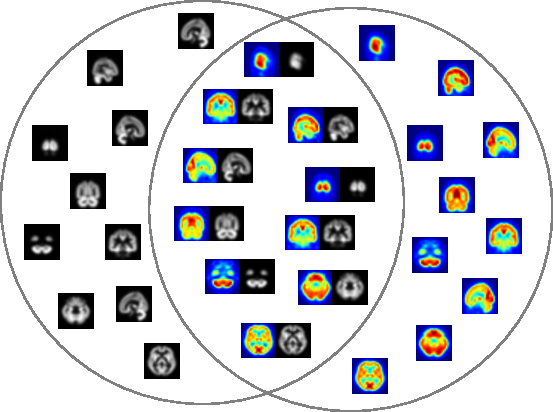
\includegraphics[width=0.8\columnwidth]{./tex/fig/nimg_scheme.pdf}
\caption{
	Pictorial example of training imaging dataset with two views, named \textit{left} and \textit{right} views.
	In this case we have 30 independent observations:
	$10$ with left-views only; $10$ with right-views only; $10$ with complete views.
	The fraction f of observations with complete views is:
	$f = 1/3$.
}
\label{fig:nimg_scheme}
\end{figure}
%
\begin{figure}[!h]
\centering
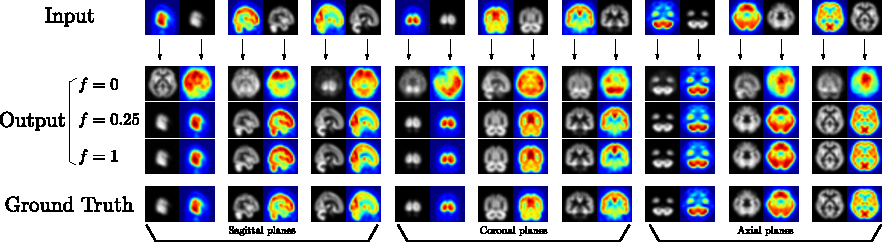
\includegraphics[width=\columnwidth]{./tex/fig/nimg_test.pdf}
\caption{
	Reconstruction of test-set digits when models are trained with an increasing fraction ($f$) of observations with complete-views.
	The left side of each digit is inferred from the input right side and \textit{vice versa}.
}
\label{fig:nimg_test}
\end{figure}

\begin{table}[h]
\centering
\caption{
	Mean squared error (MSE) and negative log-likelihood (NLL) - the lower the better -  measured as mean (st.dev) on the reconstructed brain images of the test-set.
	The MRI were used to infer the FDG slices in the same subject, and \textit{vice versa}.
	Results stratified by $f$, the fraction of observations with no missing views in the training set.
	Notice the immediate drop in the error metrics as soon as $f$ increases.
}
\label{tab:nimg}
\resizebox{\columnwidth}{!}{
	\begin{tabular}{llllll}
	\toprule
	f                &             0.00 &           0.25 &           0.50 &           0.75 &           1.00 \\
	\midrule
	MSE             &     40.72 (4.31)  &  1.77 (0.04)  &  1.63 (0.06)  &  1.54 (0.03)  &  1.51 (0.03) \\
	NLL             &    96.44 (10.33)  &  0.53 (0.09)  &  0.16 (0.12)  &  -0.07 (0.07)  &  -2.63 (0.03)  \\
	\bottomrule
	\end{tabular}
}
\end{table}


\subsection{Experiment 1: Benchmark Validation}
\begin{table}[!t]
\caption{
Mean Squared Error (MSE) of test data from adni2.
All models were trained on all the available datasets by holding-out data from the adni2 test dataset.
$5$-folds cross validation of MSE is shown as mean (standard deviation).
Best results in boldface are significant with an $\alpha$ level of 0.01 with respect to both competing methods.
}
\centering
\label{tab:model_comparison}
\begin{tabular}{lccc}
\toprule
View       &          \multicolumn{3}{c}{model}\\
           &          dae &         knn5 &           ours        \\ \cline{2-4}
clin       &  0.73 (0.14) &  0.44 (0.05) &          0.45 (0.07) \\
MRI        &  1.23 (0.31) &  0.88 (0.15) &  \textbf{0.70} (0.13) \\
FDG        &  4.20 (0.56) &  4.15 (0.59) &  \textbf{1.09} (0.15) \\
AV45       &  1.45 (0.35) &  1.20 (0.25) &  \textbf{0.89} (0.15) \\
TAU        &  1.54 (0.82) &  1.44 (0.83) &  \textbf{1.05} (0.45) \\
\bottomrule
\end{tabular}
\end{table}

% \begin{table}[!t]
% \caption{
% Add OASIS3 dataset (clin, mri, av45)
% }
% \centering
% \begin{tabular}{lcccccc}
% \toprule
% model &         clin &          mri & fdg &         av45 &          tau & mri local \\
% % model &              &              &     &              &              &            \\
% \midrule
% knn5              &  0.50 (0.06) &  0.92 (0.13) &   - &  \textbf{1.33} (0.23) &  1.10 (0.54) &  -  \\
% dae               &  0.45 (0.08) &  0.95 (0.15) &   - &  1.49 (0.20) &  1.09 (0.50) &  -  \\
% our               &  \textbf{0.39} (0.05) &  \textbf{0.75} (0.13) &   - &  1.38 (0.21) &  \textbf{0.93} (0.51) &  -  \\
% \bottomrule
% \end{tabular}
% \label{table:model_comparison}
% \end{table}
% 
% \begin{table}[!t]
% \caption{
% Add OASIS3 dataset (clin, mri, av45), ComBat normalize (mri, fdg, av45, tau)
% }
% \centering
% \begin{tabular}{lcccccc}
% \toprule
% model &         clin &          mri & fdg &         av45 &          tau & mri local \\
% % model &              &              &     &              &              &            \\
% \midrule
% knn5              &  0.51 (0.07) &  1.10 (0.17) &   - &  1.16 (0.19) &  \textbf{1.08} (0.62) &  -  \\
% dae               &  0.44 (0.06) &  1.09 (0.17) &   - &  \textbf{1.06} (0.19) &  1.45 (0.70) &  -  \\
% our               &  \textbf{0.42} (0.05) &  \textbf{0.94} (0.15) &   - &  \textbf{1.06} (0.20) &  1.32 (0.71) &  -  \\
% \bottomrule
% \end{tabular}
% \label{table:model_comparison}
% \end{table}
% 
% \begin{table}[!t]
% \caption{
% Add OASIS3 dataset (clin, mri, av45), add Geneva PET, ComBat normalize (mri, fdg, av45, tau)
% }
% \centering
% \begin{tabular}{lcccccc}
% \toprule
% model &         clin &          mri & fdg &         av45 &          tau & mri local \\
% % model &              &              &     &              &              &            \\
% \midrule
% knn5              &  0.50 (0.06) &  1.09 (0.17) &   - &  1.18 (0.20)  &  1.23 (0.92)  &  -  \\
% dae               &  0.42 (0.08) &  1.09 (0.16) &   - &  1.08 (0.19)  &  1.54 (0.87)  &  -  \\
% our               &  \textbf{0.41} (0.06) &  \textbf{0.93} (0.15) &   - &  \textbf{1.07} (0.17)  &  \textbf{1.17} (0.81)  &  -  \\
% \bottomrule
% \end{tabular}
% \label{table:model_comparison}
% \end{table}


The purpose of this experiment is to validate on real data the benchmarked results obtained with the synthetic experiments (\S~\ref{sec:synth}).

As benchmark methods, we choose the best performers on the synthetic experiments, namely KNN5 and DAE.
We choose for our model a linear Gaussian parameterization for the likelihood and variational distributions of \eqnref{eq:decoder} and \eqnref{eq:dropout_posterior} respectively.

We trained all the models (KNN5, DAE, ours) with data coming from all the datasets except from `Adni2', left out for testing purposes.
We choose the `Adni2' dataset as testing dataset since it provides all the views, and the highest number of observations per view (\tabref{table:datasets}).

Prediction performances were evaluated with the Mean Squared Error (MSE) metric, measured on the available views in the testing dataset, reconstructed with \eqnref{eq:reconstruction}.
All results were validated by means of $5$-folds cross-validation.

\paragraph{Results}
In \tabref{tab:model_comparison}, we show the MSE metric on predicting missing views in the testing dataset with our model and with the benckmark ones.
Best results are in boldface, which show a clear advantage of using our model and confirm our findings in the synthetic experiments.

\subsection{Experiment 2: Feature Prediction}
\label{ssec:feats}
% \begin{table*}
% \centering
% \caption{
% % Age Agesq.
% Mean Squared Error (MSE, the lower the better) measured on test dataset views (clinical scores and imaging derived phenotypes) predicted with our model.
% $5$-folds cross-validation results shown as as average (standard deviation).
% Models were trained on all the available views in the training dataset, independently of their presence in the testing dataset.
% Experiments run in three different conditions depending on the provenance of the training data:
% 1) `same' dataset as the testing dataset;
% 2) `different' from the testing dataset (average MSE shown);
% 3) `leave out test', from all the available datasets except the testing dataset.
% By average pooling the results (bottom) we see how in general training on data coming from multiple datasets ameliorates the results.
% }
% \label{tab:features_couple}
% \resizebox{\textwidth}{!}{
% \begin{tabular}{llcccccccccc}
% \toprule
%        & {} & \multicolumn{2}{c}{clin} & \multicolumn{2}{c}{mri} & \multicolumn{2}{c}{fdg} & \multicolumn{2}{c}{av45} & \multicolumn{2}{c}{tau} \\
%        & model\_name &        mcvae &    missmcvae &        mcvae &    missmcvae &        mcvae &    missmcvae &        mcvae &    missmcvae &        mcvae &    missmcvae \\
% \midrule
% test dataset & train dataset &              &              &              &              &              &              &              &              &              &              \\
% %\cmidrule(lr){1-2}
% adni1 & adni1 &  0.81 (0.13) &  0.79 (0.09) &  0.87 (0.12) &  0.85 (0.13) &            - &            - &            - &            - &            - &            - \\
% \cmidrule(lr){2-12}
%        & adni2 &  0.69 (0.08) &  0.71 (0.14) &  0.99 (0.17) &  0.87 (0.13) &            - &            - &            - &            - &            - &            - \\
%        & miriad &  1.16 (0.29) &  1.03 (0.28) &  1.01 (0.18) &  0.99 (0.17) &            - &            - &            - &            - &            - &            - \\
%        & geneva &            - &            - &            - &            - &            - &            - &            - &            - &            - &            - \\
%        & oasis3 &  0.63 (0.11) &  0.48 (0.05) &  0.81 (0.13) &  0.77 (0.09) &            - &            - &            - &            - &            - &            - \\
% \cmidrule(lr){2-12}
%        & all but adni1 &            - &  0.48 (0.07) &            - &  0.85 (0.16) &            - &            - &            - &            - &            - &            - \\
% \midrule
% adni2 & adni2 &  0.65 (0.10) &  0.64 (0.14) &  0.74 (0.13) &  0.69 (0.12) &  0.77 (0.13) &  0.62 (0.09) &  1.04 (0.17) &  0.81 (0.11) &  1.34 (0.60) &  1.33 (0.60) \\
% \cmidrule(lr){2-12}
%        & adni1 &  0.67 (0.13) &  0.68 (0.17) &  0.73 (0.12) &  0.74 (0.13) &            - &            - &            - &            - &            - &            - \\
%        & miriad &  0.75 (0.13) &  0.73 (0.17) &  0.77 (0.12) &  0.76 (0.12) &            - &            - &            - &            - &            - &            - \\
%        & geneva &  0.59 (0.09) &  0.50 (0.08) &            - &            - &  1.22 (0.19) &  0.92 (0.12) &  1.07 (0.17) &  0.90 (0.13) &  1.34 (0.53) &  1.04 (0.39) \\
%        & oasis3 &  0.61 (0.18) &  0.53 (0.17) &  0.71 (0.13) &  0.68 (0.11) &            - &            - &  1.34 (0.28) &  1.13 (0.24) &            - &            - \\
% \cmidrule(lr){2-12}
%        & all but adni2 &            - &  0.47 (0.10) &            - &  0.71 (0.12) &            - &  0.92 (0.11) &            - &  0.92 (0.18) &            - &  1.10 (0.34) \\
% \midrule
% geneva & geneva &  1.08 (0.46) &  1.32 (0.67) &            - &            - &  3.10 (1.12) &  2.84 (0.85) &  1.92 (0.57) &  1.81 (0.57) &  1.30 (0.74) &  1.14 (0.55) \\
% \cmidrule(lr){2-12}
%        & adni1 &            - &            - &            - &            - &            - &            - &            - &            - &            - &            - \\
%        & adni2 &  1.77 (0.77) &  1.35 (0.62) &            - &            - &  3.07 (1.08) &  2.73 (0.78) &  1.92 (0.86) &  1.33 (0.37) &  1.79 (0.78) &  1.68 (0.84) \\
%        & miriad &            - &            - &            - &            - &            - &            - &            - &            - &            - &            - \\
%        & oasis3 &  2.32 (1.40) &  1.81 (0.56) &            - &            - &            - &            - &  1.59 (0.47) &  1.54 (0.46) &            - &            - \\
% \cmidrule(lr){2-12}
%        & all but geneva &            - &  1.25 (0.59) &            - &            - &            - &  2.71 (0.80) &            - &  1.32 (0.37) &            - &  1.40 (0.55) \\
% \midrule
% miriad & miriad &  3.93 (1.60) &  3.01 (2.06) &  5.99 (1.57) &  5.95 (1.55) &            - &            - &            - &            - &            - &            - \\
% \cmidrule(lr){2-12}
%        & adni1 &  5.41 (2.54) &  4.65 (2.62) &  6.42 (1.50) &  6.47 (1.50) &            - &            - &            - &            - &            - &            - \\
%        & adni2 &  3.45 (2.16) &  1.44 (0.46) &  5.76 (1.58) &  6.05 (1.42) &            - &            - &            - &            - &            - &            - \\
%        & geneva &            - &            - &            - &            - &            - &            - &            - &            - &            - &            - \\
%        & oasis3 &  5.51 (3.63) &  4.17 (1.69) &  5.92 (1.42) &  6.01 (1.45) &            - &            - &            - &            - &            - &            - \\
% \cmidrule(lr){2-12}
%        & all but miriad &            - &  1.99 (0.68) &            - &  5.86 (1.41) &            - &            - &            - &            - &            - &            - \\
% \midrule
% oasis3 & oasis3 &  0.66 (0.16) &  0.59 (0.11) &  0.69 (0.13) &  0.68 (0.13) &            - &            - &  1.54 (0.54) &  1.27 (0.28) &            - &            - \\
% \cmidrule(lr){2-12}
%        & adni1 &  1.10 (0.19) &  1.09 (0.16) &  0.78 (0.13) &  0.79 (0.14) &            - &            - &            - &            - &            - &            - \\
%        & adni2 &  0.96 (0.18) &  1.01 (0.18) &  0.86 (0.17) &  0.75 (0.13) &            - &            - &  0.96 (0.24) &  0.98 (0.21) &            - &            - \\
%        & miriad &  1.15 (0.27) &  1.00 (0.26) &  0.87 (0.19) &  0.86 (0.17) &            - &            - &            - &            - &            - &            - \\
%        & geneva &  0.55 (0.30) &  0.42 (0.12) &            - &            - &            - &            - &  1.26 (0.58) &  1.07 (0.25) &            - &            - \\
% \cmidrule(lr){2-12}
%        & all but oasis3 &            - &  0.79 (0.14) &            - &  0.82 (0.15) &            - &            - &            - &  1.03 (0.25) &            - &            - \\
% \midrule
% \bottomrule
% \end{tabular}}
% \end{table*}
% 
% \begin{table*}
% \centering
% \caption{
% % Age
% Mean Squared Error (MSE, the lower the better) measured on test dataset views (clinical scores and imaging derived phenotypes) predicted with our model.
% $5$-folds cross-validation results shown as as average (standard deviation).
% Models were trained on all the available views in the training dataset, independently of their presence in the testing dataset.
% Experiments run in three different conditions depending on the provenance of the training data:
% 1) `same' dataset as the testing dataset;
% 2) `different' from the testing dataset (average MSE shown);
% 3) `leave out test', from all the available datasets except the testing dataset.
% By average pooling the results (bottom) we see how in general training on data coming from multiple datasets ameliorates the results.
% }
% \label{tab:features_couple2}
% \resizebox{\textwidth}{!}{
% \begin{tabular}{llcccccccccc}
% \toprule
%        & {} & \multicolumn{2}{c}{clin} & \multicolumn{2}{c}{mri} & \multicolumn{2}{c}{fdg} & \multicolumn{2}{c}{av45} & \multicolumn{2}{c}{tau} \\
%        & model\_name &        mcvae &    missmcvae &        mcvae &    missmcvae &        mcvae &    missmcvae &        mcvae &    missmcvae &        mcvae &    missmcvae \\
% test\_dataset & aggr &              &              &              &              &              &              &              &              &              &              \\
% \midrule
% adni1 & within &  0.81 (0.11) &  0.83 (0.12) &  0.89 (0.13) &  0.89 (0.12) &            - &            - &            - &            - &            - &            - \\
% \cmidrule(lr){2-12}
%        & adni2 &  0.70 (0.13) &  0.72 (0.13) &  1.00 (0.23) &  0.86 (0.12) &            - &            - &            - &            - &            - &            - \\
%        & miriad &  1.08 (0.27) &  0.95 (0.15) &  0.99 (0.17) &  0.98 (0.15) &            - &            - &            - &            - &            - &            - \\
%        & geneva &            - &            - &            - &            - &            - &            - &            - &            - &            - &            - \\
%        & oasis3 &  0.69 (0.21) &  0.47 (0.07) &  0.81 (0.13) &  0.79 (0.11) &            - &            - &            - &            - &            - &            - \\
% \cmidrule(lr){2-12}
%        & lodo &            - &  0.48 (0.08) &            - &  0.84 (0.11) &            - &            - &            - &            - &            - &            - \\
% \midrule
% adni2 & within &  0.66 (0.15) &  0.64 (0.14) &  0.74 (0.13) &  0.69 (0.12) &  0.78 (0.13) &  0.62 (0.10) &  1.05 (0.18) &  0.81 (0.12) &  1.37 (0.59) &  1.26 (0.55) \\
% \cmidrule(lr){2-12}
%        & adni1 &  0.71 (0.18) &  0.67 (0.17) &  0.73 (0.12) &  0.72 (0.12) &            - &            - &            - &            - &            - &            - \\
%        & miriad &  0.75 (0.12) &  0.71 (0.16) &  0.76 (0.12) &  0.76 (0.12) &            - &            - &            - &            - &            - &            - \\
%        & geneva &  0.58 (0.10) &  0.49 (0.07) &            - &            - &  1.20 (0.19) &  0.91 (0.12) &  1.07 (0.19) &  0.93 (0.14) &  1.36 (0.55) &  1.07 (0.44) \\
%        & oasis3 &  0.67 (0.21) &  0.52 (0.08) &  0.68 (0.11) &  0.69 (0.10) &            - &            - &  1.39 (0.38) &  1.12 (0.29) &            - &            - \\
% \cmidrule(lr){2-12}
%        & lodo &            - &  0.45 (0.07) &            - &  0.72 (0.12) &            - &  0.92 (0.13) &            - &  0.89 (0.15) &            - &  1.05 (0.36) \\
% \midrule
% geneva & within &  1.00 (0.52) &  1.39 (0.73) &            - &            - &  3.15 (1.15) &  2.87 (0.81) &  1.87 (0.53) &  1.74 (0.49) &  1.36 (0.87) &  1.12 (0.50) \\
% \cmidrule(lr){2-12}
%        & adni1 &            - &            - &            - &            - &            - &            - &            - &            - &            - &            - \\
%        & adni2 &  1.78 (0.83) &  1.40 (0.65) &            - &            - &  3.13 (1.19) &  2.77 (0.82) &  1.96 (1.02) &  1.39 (0.35) &  1.83 (0.82) &  1.57 (0.62) \\
%        & miriad &            - &            - &            - &            - &            - &            - &            - &            - &            - &            - \\
%        & oasis3 &  2.17 (1.38) &  2.56 (2.52) &            - &            - &            - &            - &  1.54 (0.45) &  1.53 (0.51) &            - &            - \\
% \cmidrule(lr){2-12}
%        & lodo &            - &  1.26 (0.72) &            - &            - &            - &  2.74 (0.83) &            - &  1.33 (0.38) &            - &  1.49 (0.62) \\
% \midrule
% miriad & within &  3.48 (1.91) &  3.77 (1.87) &  5.91 (1.55) &  5.92 (1.51) &            - &            - &            - &            - &            - &            - \\
% \cmidrule(lr){2-12}
%        & adni1 &  4.46 (3.05) &  5.10 (2.25) &  6.28 (1.56) &  6.26 (1.45) &            - &            - &            - &            - &            - &            - \\
%        & adni2 &  3.75 (1.56) &  1.73 (0.70) &  5.64 (1.57) &  5.91 (1.44) &            - &            - &            - &            - &            - &            - \\
%        & geneva &            - &            - &            - &            - &            - &            - &            - &            - &            - &            - \\
%        & oasis3 &  6.61 (5.47) &  4.24 (2.97) &  5.66 (1.40) &  6.00 (1.50) &            - &            - &            - &            - &            - &            - \\
% \cmidrule(lr){2-12}
%        & lodo &            - &  2.06 (0.76) &            - &  5.90 (1.31) &            - &            - &            - &            - &            - &            - \\
% \midrule
% oasis3 & within &  0.70 (0.18) &  0.56 (0.14) &  0.69 (0.12) &  0.68 (0.12) &            - &            - &  1.65 (0.58) &  1.32 (0.34) &            - &            - \\
% \cmidrule(lr){2-12}
%        & adni1 &  1.20 (0.28) &  1.11 (0.12) &  0.80 (0.15) &  0.78 (0.13) &            - &            - &            - &            - &            - &            - \\
%        & adni2 &  0.98 (0.16) &  0.98 (0.14) &  0.87 (0.18) &  0.75 (0.12) &            - &            - &  0.93 (0.24) &  0.99 (0.27) &            - &            - \\
%        & miriad &  1.07 (0.23) &  1.00 (0.19) &  0.86 (0.17) &  0.86 (0.17) &            - &            - &            - &            - &            - &            - \\
%        & geneva &  0.55 (0.29) &  0.40 (0.13) &            - &            - &            - &            - &  1.25 (0.54) &  1.09 (0.26) &            - &            - \\
% \cmidrule(lr){2-12}
%        & lodo &            - &  0.77 (0.15) &            - &  0.81 (0.14) &            - &            - &            - &  1.05 (0.26) &            - &            - \\
% \bottomrule
% \end{tabular}}
% \end{table*}
%
\begin{table*}
\centering
\caption{
% Age MMSE
Mean Squared Error (MSE, the lower the better) measured on test dataset views (clinical scores and imaging derived phenotypes) predicted with the Multi-Channel VAE (MCVAE) and our model (ours).
$5$-folds cross-validation results shown as as average (standard deviation).
Models were trained on all the available views in the training dataset, independently of their presence in the testing dataset.
Experiments were run in three different conditions, separated in the table by thin rules:
1) when training and testing data are chosen from the same dataset, or Single Task (ST) learning case;
2) when models trained on one dataset are tested on another dataset, or ST + Transfer Learning (TL) case;
3) when models are trained on all the available datasets except the testing one, or Multi Task Learning (MTL).
There are $12$ cases in the MTL experiments that could be fitted with our model.
In $7$ of them we measure a better performance with respect to ST cases (\S) and with respect to ST + TL cases (\dag).
In all comparable cases our model performs either similarly or statistically better than the MCVAE, with alpha levels at $0.05$ (*), $0.01$ (**), and $0.001$ (***).
}
\label{tab:features}
\resizebox{\textwidth}{!}{
\begin{tabular}{llllllllllll}
\toprule
       & view            & \multicolumn{2}{c}{clin}              & \multicolumn{2}{c}{MRI}             & \multicolumn{2}{c}{FDG}             & \multicolumn{2}{c}{AV45}            & \multicolumn{2}{c}{TAU}         \\
       & model           &        MCVAE &    ours            &        MCVAE &    ours              &        MCVAE &    ours              &        MCVAE &    ours              &        MCVAE &    ours              \\
\toprule
test dataset & train dataset &          &                    &              &                      &              &                      &              &                      &              &                      \\
\cmidrule(lr){1-2}
adni1  & adni1           &  0.90 (0.12) &  0.89 (0.13)       &  0.85 (0.11) &  0.83 (0.12)$^{*}$   &            - &            -         &            - &            -         &            - &            -         \\
\cmidrule(lr){2-12}
       & adni2           &  0.91 (0.17) &  0.77 (0.13)$^{*}$ &  1.02 (0.23) &  0.85 (0.11)$^{***}$ &            - &            -         &            - &            -         &            - &            -         \\
       & miriad          &  0.96 (0.17) &  1.14 (0.27)       &  0.80 (0.14) &  0.82 (0.13)$^{*}$   &            - &            -         &            - &            -         &            - &            -         \\
       & geneva          &            - &            -       &            - &            -         &            - &            -         &            - &            -         &            - &            -         \\
       & oasis3          &  0.83 (0.30) &  0.54 (0.10)$^{*}$ &  0.80 (0.15) &  0.76 (0.11)$^{*}$   &            - &            -         &            - &            -         &            - &            -         \\
\cmidrule(lr){2-12}
       & all but adni1   &            - &  0.45 (0.07)\S\dag &            - &  0.77 (0.10)\S       &            - &            -         &            - &            -         &            - &            -         \\
\toprule
adni2 & adni2            &  0.83 (0.11) &  0.73 (0.15)       &  0.74 (0.13) &  0.70 (0.11)$^{**}$  &  0.73 (0.14) &  0.59 (0.10)$^{***}$ &  1.03 (0.19) &  0.80 (0.10)$^{***}$ &  1.33 (0.59) &  1.18 (0.52)$^{*}$   \\
\cmidrule(lr){2-12}
       & adni1           &  0.77 (0.18) &  0.80 (0.14)       &  0.74 (0.11) &  0.75 (0.12)         &            - &            -         &            - &            -         &            - &            -         \\
       & miriad          &  0.73 (0.20) &  0.71 (0.18)       &  0.78 (0.13) &  0.77 (0.13)         &            - &            -         &            - &            -         &            - &            -         \\
       & geneva          &  0.47 (0.06) &  0.48 (0.09)       &            - &            -         &  1.40 (0.21) &  1.09 (0.15)$^{***}$ &  1.10 (0.21) &  0.91 (0.15)$^{**}$  &  1.34 (0.52) &  1.05 (0.45)$^{***}$ \\
       & oasis3          &  0.76 (0.23) &  0.61 (0.13)       &  0.68 (0.12) &  0.68 (0.11)         &            - &            -         &  1.32 (0.29) &  1.13 (0.26)$^{***}$ &            - &            -         \\
\cmidrule(lr){2-12}
       & all but adni2   &            - &  0.45 (0.07)\S\dag &            - &  0.70 (0.13)         &            - &            -         &            - &  0.89 (0.15)\dag     &            - &            -         \\
\toprule
geneva & geneva          &  0.79 (0.34) &  0.98 (0.52)       &            - &            -         &  3.63 (1.35) &  3.18 (1.04)$^{*}$   &  1.82 (0.57) &  1.76 (0.47)$^{*}$   &  1.27 (0.82) &  1.19 (0.67)$^{*}$   \\
\cmidrule(lr){2-12}
       & adni1           &            - &            -       &            - &            -         &            - &            -         &            - &            -         &            - &            -         \\
       & adni2           &  2.57 (1.09) &  2.07 (1.05)       &            - &            -         &  3.01 (1.05) &  2.69 (0.77)$^{*}$   &  1.92 (0.90) &  1.41 (0.39)         &  1.81 (0.81) &  1.42 (0.66)$^{***}$ \\
       & miriad          &            - &            -       &            - &            -         &            - &            -         &            - &            -         &            - &            -         \\
       & oasis3          &  1.93 (0.66) &  2.28 (0.89)       &            - &            -         &            - &            -         &  1.70 (0.51) &  1.63 (0.55)$^{*}$   &            - &            -         \\
\cmidrule(lr){2-12}
       & all but geneva  &            - &  1.80 (1.16)\dag   &            - &            -         &            - &            -         &            - &  1.35 (0.37)\S\dag   &            - &            -         \\
\toprule
miriad & miriad          &  3.21 (1.07) &  3.23 (2.55)       &  6.39 (1.57) &  6.38 (1.52)         &            - &            -         &            - &            -         &            - &            -         \\
\cmidrule(lr){2-12}
       & adni1           &  6.90 (3.33) &  6.49 (3.42)       &  6.60 (1.61) &  6.73 (1.55)         &            - &            -         &            - &            -         &            - &            -         \\
       & adni2           &  5.60 (2.76) &  3.97 (3.14)       &  5.93 (1.90) &  6.59 (1.64)         &            - &            -         &            - &            -         &            - &            -         \\
       & geneva          &            - &            -       &            - &            -         &            - &            -         &            - &            -         &            - &            -         \\
       & oasis3          &  6.80 (6.52) &  6.24 (4.62)       &  6.29 (1.68) &  6.23 (1.40)         &            - &            -         &            - &            -         &            - &            -         \\
\cmidrule(lr){2-12}
       & all but miriad  &            - &  2.31 (1.65)\S\dag       &            - &  6.17 (1.37)\S\dag   &            - &            -         &            - &            -         &            - &            -         \\
\toprule
oasis3 & oasis3          &  0.83 (0.33) &  0.68 (0.28)       &  0.68 (0.13) &  0.66 (0.12)$^{*}$   &            - &            -         &  1.58 (0.63) &  1.22 (0.26)$^{***}$ &            - &            -         \\
\cmidrule(lr){2-12}
       & adni1           &  1.20 (0.25) &  1.23 (0.28)       &  0.78 (0.14) &  0.79 (0.14)         &            - &            -         &            - &            -         &            - &            -         \\
       & adni2           &  1.11 (0.33) &  1.09 (0.24)       &  0.89 (0.18) &  0.76 (0.15)$^{***}$ &            - &            -         &  0.94 (0.22) &  1.02 (0.26)$^{*}$   &            - &            -         \\
       & miriad          &  0.98 (0.21) &  1.02 (0.20)       &  0.83 (0.18) &  0.83 (0.18)         &            - &            -         &            - &            -         &            - &            -         \\
       & geneva          &  0.55 (0.28) &  0.49 (0.26)       &            - &            -         &            - &            -         &  1.23 (0.61) &  1.11 (0.26)$^{*}$   &            - &            -         \\
\cmidrule(lr){2-12}
       & all but oasis3  &            - &  0.72 (0.09)       &            - &  0.81 (0.15)         &            - &            -         &            - &  1.09 (0.30)\S       &            - &            -         \\
\bottomrule
\end{tabular}}
\end{table*}

The purpose of this experiment is to compare, in features prediction experiments, the generalization performance the MCVAE model with respect to our new Multi Task extension (MT-MCVE).
This experiment was run in three different conditions:
%
\begin{enumerate}
\item Single Task with Internal Benchmark (STIB): when training and testing data are chosen from the same dataset;
%
\item Single Task with External Benchmark (STEB): when models trained on one dataset are tested on another one;
%
\item Multi Task Learning (MTL): when models are trained on all the available datasets except the testing one.
%
\end{enumerate}
%
In STIB and STEB experiments, both MCVAE and MT-MCVAE models are trained on the same views,
but while in MCVAE we need to discard observations with missing views from the training set,
with MT-MCVAE we can include them by grouping together observations with common views into homogeneous tasks.
In MTL experiments, MCVAE models cannot be trained because no observation has simultaneously all the views.
%By removing the cases where views are not simultaneously present in both the training and testing set,
%we are left with $16$ possible scenarios where all the three experimental conditions can be simultaneously tested an thus compared.

We choose for both MCVAE and MT-MCVAE a linear Gaussian parameterization for the likelihood and variational distributions as in \eqnref{eq:decoder} and \eqnref{eq:dropout_posterior} respectively.
Models were trained on all the available views in the training dataset. %, independently of their presence in the testing dataset.
Prediction performances were evaluated with the Mean Squared Error (MSE) metric, measured on the available views in the testing dataset, reconstructed with \eqnref{eq:reconstruction}.
All results were validated by means of $5$-folds cross-validation.

\begin{table}
\centering
\caption{
	Mean Squared Reconstruction Error (the lower the better) measured on clinical scores and imaging derived phenotypes predicted with our model.
	Results stratified by the number of layers in the encoder-decoder architecture.
}
\label{tab:features_mtl_nl}
\resizebox{\columnwidth}{!}{
\begin{tabular}{lllll}
\toprule
\#layers &            1 &            2 &            3 &            4 \\
\midrule
clin    &  0.97 (0.49) &  1.05 (0.65) &  1.04 (0.60) &  1.02 (0.50) \\
MRI     &  2.09 (0.92) &  2.14 (0.69) &  2.13 (0.68) &  2.13 (0.68) \\
AV45    &  1.09 (0.29) &  1.16 (0.25) &  1.15 (0.26) &  1.15 (0.25) \\
\bottomrule
\end{tabular}
}
\end{table}


\paragraph{Results}
In \tabref{tab:features} and \tabref{tab:features_mtl} we show the prediction error in terms of MSE for each test dataset and view, on the three experimental conditions described earlier.
In STIB and STEB cases \tabrefp{tab:features}, the MT-MCVAE model performs either similarly or statistically better than the MCVAE, especially in cases where the difference between the union and intersection set of observations is higher (cfr. \tabref{table:datasets}).
In the MTL scenario \tabrefp{tab:features_mtl} there are $12$ cases that could be fitted with MT-MCVAE only.
We measure an overall better performance of MTL with respect to STIB ($7/12$ of cases) and with respect to STEB ($10/12$ of cases).

\subsection{Experiment 3: Diagnosis Prediction}
\label{ssec:classifier}
% \begin{table*}
% \centering
% \caption{
% Experiment of diagnosis classification.
% Classification accuracy (the higher the better) from a 5-folds cross-validation experiments is shown.
% On average, in-dataset (same) prediction performance is higher with respect to all other cases.
% Out-dataset prediction performance is higher if multiple dataset are pooled together (leave out test) with respect to the 
% average case where our model is trained with a single dataset (different).
% }
% \label{tab:dx_couples}
% \begin{tabular}{llllllll}
% \toprule
%        & classification\_test & \multicolumn{2}{l}{AD\_vs\_MCI} & \multicolumn{2}{l}{AD\_vs\_NC} & \multicolumn{2}{l}{MCI\_vs\_NC} \\
%        & model\_name &          mcvae &      missmcvae &          mcvae &      missmcvae &         mcvae &     missmcvae \\
% test\_dataset & aggr &                &                &                &                &               &               \\
% \midrule
% adni1 & within &   72.70 (3.72) &   72.87 (4.37) &   81.69 (2.97) &   81.51 (3.14) &  62.00 (8.91) &  62.90 (8.72) \\
%        & cross &   47.04 (5.88) &  47.74 (12.56) &  66.55 (15.29) &   72.30 (8.90) &  53.12 (6.42) &  59.65 (2.76) \\
%        & lodo &   50.09 (4.75) &   56.17 (4.29) &   66.55 (6.48) &   74.48 (3.06) &  53.12 (6.42) &  59.65 (2.76) \\
% adni2 & within &   50.58 (3.90) &   80.07 (2.53) &   82.86 (3.28) &   87.92 (3.46) &  58.63 (4.27) &  65.56 (1.11) \\
%        & cross &   61.04 (4.49) &   61.11 (4.21) &   67.59 (5.27) &   70.04 (6.55) &  63.05 (2.00) &  62.75 (1.80) \\
%        & lodo &              - &   68.46 (1.31) &   66.28 (4.35) &   83.89 (1.93) &  63.05 (2.00) &  62.75 (1.80) \\
% geneva & within &   65.76 (3.62) &   77.70 (8.12) &              - &              - &             - &             - \\
%        & cross &  33.89 (11.88) &  50.09 (21.50) &              - &              - &             - &             - \\
%        & lodo &  42.42 (14.70) &   56.70 (4.13) &              - &              - &             - &             - \\
% miriad & within &              - &              - &  83.85 (13.84) &  86.70 (15.68) &             - &             - \\
%        & cross &              - &              - &  64.95 (19.72) &  73.04 (15.31) &             - &             - \\
%        & lodo &              - &              - &  61.76 (18.25) &   92.53 (0.30) &             - &             - \\
% oasis3 & within &              - &              - &   74.47 (2.49) &   80.35 (3.59) &             - &             - \\
%        & cross &              - &              - &  60.50 (10.39) &  61.89 (13.23) &             - &             - \\
%        & lodo &              - &              - &   68.05 (6.41) &   75.43 (5.67) &             - &             - \\
% \bottomrule
% \end{tabular}
% \end{table*}

\begin{table}
\centering
\caption{
Number of subjects stratified by dataset and diagnosis:
Alzheimer's Disease (AD);
Mild Cognitive Impairment (MCI);
Normal Cognition (NC).
}
\label{tab:dx_stratification}
\begin{tabular}{lccccc}
\toprule
   &     AD &    MCI &     NC &  other & total \\
\midrule
adni1   &  403 &  172 &  165 &   -  &  740 \\
adni2   &  328 &  455 &  541 &   -  & 1324 \\
geneva  &  147 &  405 &    - &  447 &  999 \\
miriad  &   44 &   -  &   23 &   -  &   67 \\
oasis3  &  149 &    - &  380 &   -  &  529 \\
\bottomrule
\end{tabular}
\end{table}


\begin{table*}
\centering
\caption{
Experiment of diagnosis classification run with the Multi-Channel VAE (MCVAE) and our model (ours).
$5$-folds classification accuracy in $\%$ is shown as mean (standard deviation). 
Since there are no MCI in miriad and oasis3 datasets, the classification tests `AD vs MCI' and `MCI vs NC' are meaningless and not reported.
Since there are no NC in the geneva dataset, the classification tests `AD vs NC' and `MCI vs NC' are meaningless and not reported.
Experiments were run in three different conditions, separated in the table by thin rules:
1) when training and testing data are chosen from the same dataset, or Single Task (ST) learning case;
2) when models trained on one dataset are tested on another dataset, or ST + Transfer Learning (TL) case;
3) when models are trained on all the available datasets except the testing one, or Multi Task Learning (MTL).
There are $7$ cases in the MTL condition that could be fitted with our model, which is not possible to do with the MCVAE.
In $5$ of them (\dag) we measure on average a better performance with respect to the second condition.
In all the cases where the classification accuracy is $>50\%$ our model performs either similarly or statistically better than the MCVAE, with $\alpha$ levels at $0.05$ (*), $0.01$ (**), and $0.001$ (***).
}
\label{tab:classifier}
\resizebox{\textwidth}{!}{
\begin{tabular}{llllllll}
\toprule
       & classification task    & \multicolumn{2}{c}{AD vs MCI} & \multicolumn{2}{c}{AD vs NC} & \multicolumn{2}{c}{MCI vs NC} \\
       & model          & \multicolumn{1}{c}{mcvae}  & \multicolumn{1}{c}{ours} & \multicolumn{1}{c}{mcvae}  & \multicolumn{1}{c}{ours} & \multicolumn{1}{c}{mcvae}  & \multicolumn{1}{c}{ours} \\
\toprule
test dataset & train dataset &                 &                        &                &                       &               &                       \\
\cmidrule(lr){1-2}
adni1  & adni1          &   72.70 (3.72)       &  72.87 (4.37)          &   81.69 (2.97) &   81.51 (3.14)        &  62.00 (8.91) &  62.90 (8.72)         \\
\cmidrule(lr){2-8}
       & adni2          &   47.48 (3.56)       &  58.96 (3.55)$^{***}$  &   68.50 (4.86) &   73.77 (2.80)$^{*}$  &  53.12 (6.42) &  59.65 (2.76)$^{*}$   \\
       & miriad         &              -       &             -          &   82.58 (4.75) &   80.82 (3.16)        &             - &             -         \\
       & oasis3         &              -       &             -          &   48.57 (6.48) &   62.31 (6.43)$^{**}$ &             - &             -         \\
       & geneva         &   46.61 (8.03)$^{*}$ &  36.52 (5.29)          &              - &              -        &             - &             -         \\
\cmidrule(lr){2-8}
       & all but adni1  &  -                   &  56.17 (4.29)          &  -             &   74.48 (3.06)\dag    &  -            &             -         \\
\toprule
adni2  & adni2          &   50.58 (3.90)       &  80.07 (2.53)$^{***}$  &   82.86 (3.28) &   87.92 (3.46)$^{*}$  &  58.63 (4.27) &  65.56 (1.11)$^{**}$  \\
\cmidrule(lr){2-8}
       & adni1          &   57.59 (2.61)       &  58.23 (2.87)          &   64.21 (3.36) &   64.21 (3.52)        &  63.05 (2.00) &  62.75 (1.80)         \\
       & miriad         &              -       &             -          &   70.32 (7.29) &   70.20 (7.17)        &             - &             -         \\
       & oasis3         &              -       &             -          &   68.24 (2.97) &   75.72 (1.90)$^{**}$ &             - &             -         \\
       & geneva         &   64.49 (2.98)       &  63.98 (3.30)          &              - &              -        &             - &             -         \\
\cmidrule(lr){2-8}
       & all but adni2  &              -       &  68.46 (1.31)\dag       &   -            &   83.89 (1.93)\dag    &  -            &             -         \\
\toprule
geneva & geneva         &   65.76 (3.62)       &  77.70 (8.12)$^{*}$    &              - &              -        &             - &             -         \\
\cmidrule(lr){2-8}
       & adni1          &   29.17 (5.87)       &  30.08 (5.49)          &              - &              -        &             - &             -         \\
       & adni2          &  38.61 (15.08)       &  70.11 (2.90)$^{**}$   &              - &              -        &             - &             -         \\
\cmidrule(lr){2-8}
       & all but geneva &              -       &  56.70 (4.13) &               -         &              -        &             - &             -         \\
\toprule
miriad & miriad         &              -       &             -          &  83.85 (13.84) &  86.70 (15.68)        &             - &             -         \\
\cmidrule(lr){2-8}
       & adni1          &              -       &             -          &  74.18 (14.37) &  74.18 (14.37)        &             - &             -         \\
       & adni2          &              -       &             -          &  74.95 (11.58) &  78.90 (11.54)$^{*}$  &             - &             -         \\
       & oasis3         &              -       &             -          &  45.71 (18.08) &  66.04 (19.35)        &             - &             -         \\
\cmidrule(lr){2-8}
       & all but miriad &              -       &             -          &  -             &  92.53 (0.30)\dag     &             - &             -         \\
\toprule
oasis3 & oasis3         &              -       &             -          &   74.47 (2.49) &   80.35 (3.59)$^{*}$  &             - &             -         \\
\cmidrule(lr){2-8}
       & adni1          &              -       &             -          &   49.16 (6.34) &   48.22 (5.78)        &             - &             -         \\
       & adni2          &              -       &             -          &   67.86 (3.80) &   75.42 (4.68)$^{*}$  &             - &             -         \\
       & miriad         &              -       &             -          &   64.48 (8.65) &   62.02 (9.74)        &             - &             -         \\
\cmidrule(lr){2-8}
       & all but oasis3 &              -       &             -          &   -            &   75.43 (5.67)\dag    &             - &             -         \\
\bottomrule
\end{tabular}}
\end{table*}


The purpose of this experiment is to compare, in diagnosis prediction experiments, the generalization performance of the MCVAE model with respect to the MT-MCVAE,
in the three experimental conditions described earlier: STIB, STEB, and MTL.
%
Diagnostic classes are:
Alzheimer's disease (AD),
mild cognitive impairment (MCI),
normal cognition (NC).

For both MCVAE and MT-MCVAE we choose a linear Gaussian parameterization for the variational distributions as in \eqnref{eq:dropout_posterior}.
To adapt the models to this new classification experiment, we adopt as decoding function for the latent variable $\z$, the following Categorical likelihood:
\begin{align}
\label{eq:classifier}
\p{y_{d,n}|\z,\thetab} = \operatorname{Cat}\left(\mathbf{\pi}=\thetab\z\right),
\end{align}
where $y_{d,n}$ is the diagnosis associated to the data-point $n$ in the dataset $d$.
The probability vector $\mathbf{\pi}$ is a two dimensional vector representing the class probability for each of the three binary comparisons across the three diagnostic classes, namely AD \textit{vs} MCI, AD \textit{vs} NC, MCI \textit{vs} NC ,and is parametrized with a linear transformation of the latent $\z$ by the matrix $\thetab$.

Models were trained on all the available views in the training dataset, independently of their presence in the testing dataset.
Classes probabilities were inferred from the all the available views in the testing dataset with the following equation:
\begin{equation}\label{eq:reconstructiony}
\begin{aligned}
\hat{y}_{d,n} = \frac{1}{V_{d, n}} \sum_{w=1}^{V_{d, n}} \EE{q_{d,n,w}(\z)}{\p{y_{d,n}|\z,\thetab}}.
\end{aligned}
\end{equation}
We attributed to each subject the diagnostic class with the highest inferred probability.

The performance on test datasets was evaluated by measuring the classification accuracy (\%).
All results were validated by means of $5$-folds cross-validation.

\paragraph{Results}
In \tabref{tab:classifier} we show the classification accuracy of MCVAE and MT-MCVAE.
In STIB and STEB cases, the MT-MCVAE model performs either similarly or statistically better than the MCVAE.
There are $7$ cases in the MTL condition \tabrefp{tab:classifier_mtl} that could be fitted with the MT-MCVAE model only.
In all of them we measure a better performance with respect to the best STEB cases.

